% This is "sig-alternate.tex" V2.0 May 2012
% This file should be compiled with V2.5 of "sig-alternate.cls" May 2012
%
% This example file demonstrates the use of the 'sig-alternate.cls'
% V2.5 LaTeX2e document class file. It is for those submitting
% articles to ACM Conference Proceedings WHO DO NOT WISH TO
% STRICTLY ADHERE TO THE SIGS (PUBS-BOARD-ENDORSED) STYLE.
% The 'sig-alternate.cls' file will produce a similar-looking,
% albeit, 'tighter' paper resulting in, invariably, fewer pages.
%
% ----------------------------------------------------------------------------------------------------------------
% This .tex file (and associated .cls V2.5) produces:
%       1) The Permission Statement
%       2) The Conference (location) Info information
%       3) The Copyright Line with ACM data
%       4) NO page numbers
%
% as against the acm_proc_article-sp.cls file which
% DOES NOT produce 1) thru' 3) above.
%
% Using 'sig-alternate.cls' you have control, however, from within
% the source .tex file, over both the CopyrightYear
% (defaulted to 200X) and the ACM Copyright Data
% (defaulted to X-XXXXX-XX-X/XX/XX).
% e.g.
% \CopyrightYear{2007} will cause 2007 to appear in the copyright line.
% \crdata{0-12345-67-8/90/12} will cause 0-12345-67-8/90/12 to appear in the copyright line.
%
% ---------------------------------------------------------------------------------------------------------------
% This .tex source is an example which *does* use
% the .bib file (from which the .bbl file % is produced).
% REMEMBER HOWEVER: After having produced the .bbl file,
% and prior to final submission, you *NEED* to 'insert'
% your .bbl file into your source .tex file so as to provide
% ONE 'self-contained' source file.
%
% ================= IF YOU HAVE QUESTIONS =======================
% Questions regarding the SIGS styles, SIGS policies and
% procedures, Conferences etc. should be sent to
% Adrienne Griscti (griscti@acm.org)
%
% Technical questions _only_ to
% Gerald Murray (murray@hq.acm.org)
% ===============================================================
%
% For tracking purposes - this is V2.0 - May 2012

\documentclass{sig-alternate}
\usepackage{algorithm}
\usepackage {mathpartir}
\begin{document}
%
% --- Author Metadata here ---
\conferenceinfo{WOODSTOCK}{'97 El Paso, Texas USA}
%\CopyrightYear{2007} % Allows default copyright year (20XX) to be over-ridden - IF NEED BE.
%\crdata{0-12345-67-8/90/01}  % Allows default copyright data (0-89791-88-6/97/05) to be over-ridden - IF NEED BE.
% --- End of Author Metadata ---

\title{Detecting Android Malware Through Inter-Component Call Graph}
\subtitle{[Extended Abstract]
\titlenote{A full version of this paper is available as
\textit{Author's Guide to Preparing ACM SIG Proceedings Using
\LaTeX$2_\epsilon$\ and BibTeX} at
\texttt{www.acm.org/eaddress.htm}}}
%
% You need the command \numberofauthors to handle the 'placement
% and alignment' of the authors beneath the title.
%
% For aesthetic reasons, we recommend 'three authors at a time'
% i.e. three 'name/affiliation blocks' be placed beneath the title.
%
% NOTE: You are NOT restricted in how many 'rows' of
% "name/affiliations" may appear. We just ask that you restrict
% the number of 'columns' to three.
%
% Because of the available 'opening page real-estate'
% we ask you to refrain from putting more than six authors
% (two rows with three columns) beneath the article title.
% More than six makes the first-page appear very cluttered indeed.
%
% Use the \alignauthor commands to handle the names
% and affiliations for an 'aesthetic maximum' of six authors.
% Add names, affiliations, addresses for
% the seventh etc. author(s) as the argument for the
% \additionalauthors command.
% These 'additional authors' will be output/set for you
% without further effort on your part as the last section in
% the body of your article BEFORE References or any Appendices.

\numberofauthors{8} %  in this sample file, there are a *total*
% of EIGHT authors. SIX appear on the 'first-page' (for formatting
% reasons) and the remaining two appear in the \additionalauthors section.
%
\author{
% You can go ahead and credit any number of authors here,
% e.g. one 'row of three' or two rows (consisting of one row of three
% and a second row of one, two or three).
%
% The command \alignauthor (no curly braces needed) should
% precede each author name, affiliation/snail-mail address and
% e-mail address. Additionally, tag each line of
% affiliation/address with \affaddr, and tag the
% e-mail address with \email.
%
% 1st. author
\alignauthor
Yu Feng\\
       \affaddr{College of William \& Mary}\\
       \email{yufeng@cs.wm.edu}
% 2nd. author
\alignauthor
Saswat Anand\\
       \affaddr{Stanford University}\\
       \email{saswat@cs.stanford.edu}
% 3rd. author
\alignauthor Isil Dillig\\
       \affaddr{Microsoft Research Cambridge}\\
       \email{idillig@gmail.com}
%\and  % use '\and' if you need 'another row' of author names
}
% There's nothing stopping you putting the seventh, eighth, etc.
% author on the opening page (as the 'third row') but we ask,
% for aesthetic reasons that you place these 'additional authors'
% in the \additional authors block, viz.
\additionalauthors{Additional authors: John Smith (The Th{\o}rv{\"a}ld Group,
email: {\texttt{jsmith@affiliation.org}}) and Julius P.~Kumquat
(The Kumquat Consortium, email: {\texttt{jpkumquat@consortium.net}}).}
\date{30 July 1999}
% Just remember to make sure that the TOTAL number of authors
% is the number that will appear on the first page PLUS the
% number that will appear in the \additionalauthors section.

\maketitle
\begin{abstract}
As smartphones have become ubiquitous in a tremendous speed, the security problem of Android applications becomes urgent, especially the solution to protect user's privacy data from being stealing by malicious applications. Many researchers have been working on this  problem for years. Meanwhile the malware families also keep on evolving. Some of them are hard to detect even using the state of the art tools while others can be detected by requiring a lot of manual effort. We need to come up with a way to quantify the semantic behavior of Android application and understand how those applications are compromised.

In this paper, we propose Inter-Component Call Graph(ICCG), which is a high level abstraction of Android application describing how components are connected together. We also present a query language on ICCG to detect malicious applications that match existing families.  The basic idea is, given an Android application, we apply tainted analysis on it and generate its ICCG.  Then we plot each source and sink to its corresponding component. By studying the behavior of  some sample malware we extract a subgraph that corresponds to the malicious components. Finally we formalize the semantic behavior of malicious components into a query criteria and apply it to the application we want to check. If there exists a match, the application is malicious, otherwise we conclude the application does not belong to the malware family we want to check. We apply our tool to 1000 malicious applications from 9 major families and we found 90\% of them successfully.  We also run the tool on 10,000 applications from Google Play and we get a low false positive.

\end{abstract}

% A category with the (minimum) three required fields
%\category{H.4}{Information Systems Applications}{Miscellaneous}
%A category including the fourth, optional field follows...
%\category{D.4.6}{Software Engineering}{Metrics}[complexity measures, performance measures]
\category{D.4.6}{Software Engineering}{Security and Protection}

\terms{Security}

\keywords{Android Malware, Smartphone Security, Static Analysis, Tainted Analysis}

\section{Introduction}
Smartphones are becoming ubiquitous. According to the keynote of Goole 2013 I/O meeting, there have been more than 900 million Android activations in total and 48 billion apps have been downloaded on Android. 2.5 billion applications are installed every month either from Google Play or other third-party's markets.  At the same time, the task of malware detection becomes critical and many researchers have worked on this area. Zhou, Wu, et al[7] used program dependent graph(PDG) to detect the extraneous codes that are packaged to the original applications.

In this paper, we propose Inter-Component Call Graph(ICCG), which is a high level abstraction of Android application describing how components are connected together. We also present a query language on ICCG to detect malicious applications that match existing families.  The basic idea is, given an Android application, we apply tainted analysis on it and generate its ICCG.  Then we plot each source and sink to its corresponding component. By studying the behavior of  some sample malware we extract a subgraph that corresponds to the malicious components. Finally we formalize the semantic behavior of malicious components into a query criteria and apply it to the application we want to check. If there exists a match, the application is malicious, otherwise we conclude the application does not belong to the malware family we want to check. We apply our tool to 1000 malicious applications from 9 major families and we found 90\% of them successfully.  We also run the tool on 10,000 applications from Google Play and we get a low false positive.

\subsection{Problem Definition and Approach}
Here are three problems we are trying to solve: First, how to come up with a abstraction for Android application that summarizes the its overall information. Second, how to formalize the behavior of  real world malware families in terms of the representation of ICCG. Third, how to combine previous two  together to detect malware.

\begin{figure}
\begin{center}
  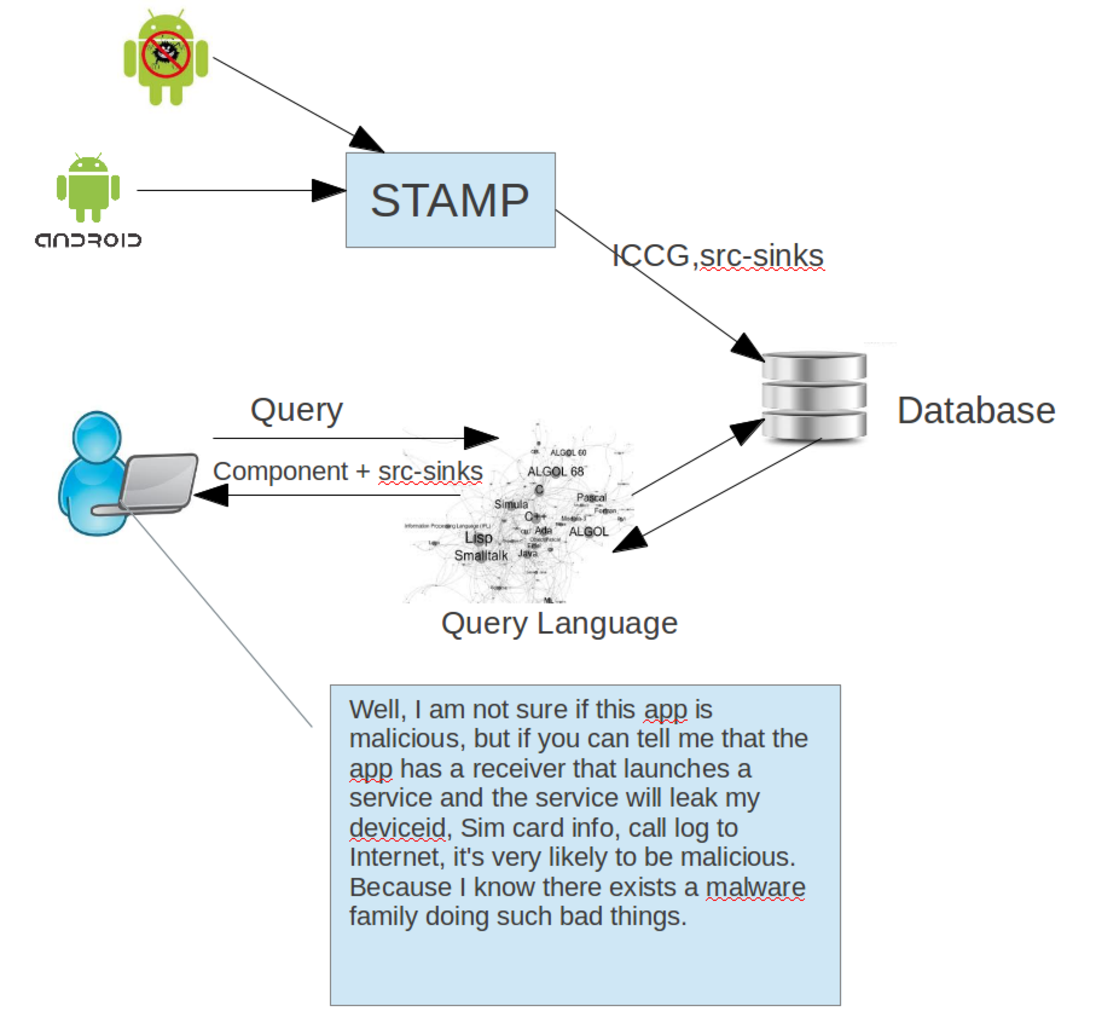
\includegraphics[scale=0.5]{img/overview}
\end{center}
\caption{Overview of Approach.}
\label{fig-ffsm}
\end{figure}



\subsection{Overview and running example}
Figure 2 is an ICCG of malicious components in DroidDreamLight family which is packaged to several applications in Google Play and other markets. We will use it through the whole paper to illustrate our technique. The upper part is ICCG while lower part are the corresponding declaration in AndroidManifest.xml. The malicious behavior of this family looks like this: first, it registers a receiver which is launched by Android framework as soon as it captures  "PHONE\_STATE" event; Then the receiver will launch a service component;  Finally the service component will read user's device information, SDK version and leak them to internet.
\begin{figure}
\begin{center}
  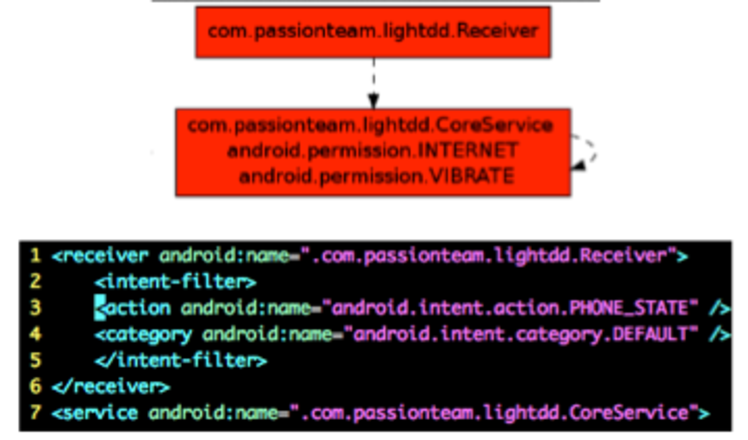
\includegraphics[scale=0.7]{img/example}
\end{center}
\caption{A sample of malware in DriodDreamLight family.}
\label{fig-ffsm}
\end{figure}

In order to detect this malicious application, we need to quantify the semantic behavior of its corresponding family. Figure 1 describes the overview approach of our technique: For each application, first we generate its 
ICCG and perform tainted analysis on it. Second, we compute the legacy of each component. The legacy can be any information that helps to quantify the behavior of a malware. e.g, source-sink flow, dangerous method invocation, suspicious intent filter, etc. Third, we study the specification of a specific malware family. In this example, we look into the document of DroidDreamLight family[9] and formalize its behavior to a query. Finally we apply the query to our database which records the information of current application's ICCG and check whether there exists a match. If yes, our tool concludes that current application is malicious, otherwise it does not belong to the malware family we want to check.

Our approach is based on the following insights:
\begin{itemize}
  \item We can not assert an application is malicious only because we find a source-sink. But most of malicious applications usually produce a lot of source-sinks such as device information, network information, SDK version etc;
    \item Most of the samples under the same malware family will share a similar subgraph in our ICCG and those information can be used as a semantic signature of corresponding malware family.
\end{itemize}

\subsection{Organization and Contributions}
The rest of the paper is organized as follows: Section 2 introduces some basic concepts of Android application; Section 3 describes the methodology of our technique; Section 4 brings up some implementation about our tool and Section 5 presents our experimental results; Section 6 performs a case study on a real world malware; Section 7 surveys some related work and section 8 makes the conclusion. In summary, this paper makes the following contributions:
\begin{itemize}
  \item We come up with the concept of Inter-component Call graph(ICCG), which is a new abstraction of Android application; 
    \item We come up with a query language to formalize the semantic of malware behavior.
  \item  We systematically study the behavior of 9 major malware families and successfully detect 90\% of them in Genome project[6], a malware benchmark collecting most of the malware during 2010 to 2011.
\end{itemize}

\section{Background}

\subsection{Android Background}
Android has a complicated message passing system where Intents are used to link the connections among multiple components.  We can think of intent as an object which can invoke remote methods. Intent is used both in inter- and intra-applications.

In real world, intent can be used as explicit or implicit communication. Explicit means that developer specifies a target component that will be invoked by name, whereas  implicit intent can invoke any remote component satisfied its specification, and usually this is achieved by declaring an intent filter, which contains action name, category and data. 

Intents are delivered to components in Android framework. There are four kinds of components:
\begin{itemize}
  \item \emph{Activities} represent user interface. An activity usually starts with a Intent, and return data upon completion. 
  \item \emph{Services} represent background operations that do not have user interface. A component can start, bind and stop a service through the support of Intents.
  \item \emph{Broadcast receivers} are used to register for system or application events. All registered receivers for an event will be invoked by the android runtime once the event happens.
  \item \emph{Content Providers} manage access to a structured set of data. They are used for both persistent internal data and as a way for data sharing between applications.
\end{itemize}

\section{Methodology}
In this section, first we present a simple language which help us to formalize our technique. Then we describe the design of ICCG construction and how to compute the legacy of each component. Finally we formalize the behavior of malware in terms of a query language.

\begin{figure}

A.java:  \\
      1 public class A extends Activity \{   \\
      2   \hspace{4pt}   protected void onCreate() \{ \\
      3  \hspace{8pt}        Intent intent = new Intent(); \\
      4      \hspace{8pt}     intent.setClass(B.class); \\
     5   \hspace{8pt}       foo.start(intent);  \\
     6    \hspace{4pt}  \}   \\
     7 \}   \\
     
      1 public class foo \{   \\
      2   \hspace{4pt}   public static void start(Intent i) \{ \\
     3  \hspace{8pt}       startActivity(i);  \\
     4    \hspace{4pt}  \}   \\
     5 \}   \\
     
           1 public class Intent \{   \\
      2   \hspace{4pt}   public static string componentName; \\
     4    \hspace{4pt} ......   \\
     5 \}   \\

\caption{Code example to illustrate our approach.}
\label{fig-ffsm}
\end{figure}

\subsection{Language}
In this section, as Figure 4 shown, we give a simple imperative call-by-value language which will be used throughout the write-up to formalize our technique. 
In this language, one program will have a set of classes and each class $c$ consists of a set of methods. Each method $m$ contains a body, which consists of several statements $s$.  

\begin{figure}
\begin{center}
\[
\begin{array}{rl}
{\rm Program \ P} &:=  c^* \\
{\rm Class \ C} &:=  m^* \\
{\rm Method \  m:} &:= \text{def} \ m = \{k\} \\
{\rm  Stmt \ s:} &:= skip  \\
                                & | \ k_1; k_2 | \text{ if }(*) \text{ then } k_1 \text{ else } k_2 \\
                                & | \  \text{while}(*) \ do \ \{S\}\\
 {\rm New Statement \:} &:= y=new X  \\
{\rm Assignment \ :} &:= y=x  \\
{\rm Load \ } &:=y = x.f \\
{\rm Store \ } &:= y.f = x \\
{\rm Return \ } &:= \text{ return } y \\
{\rm  Invocations \ :} &:= m(v_1, v_2,...)
\end{array}
\]
\end{center}
\caption{Language used for formal development}
\label{fig-ffsm}
\end{figure}

\subsection{ICCG Construction}
In order to compute a precise ICCG, we perform a K-object sensitive on-the-fly call graph construction. The basic idea is, we perform both call graph construction and K-object sensitive points-to analysis simultaneously until both of two reach a fixed point. The idea of K-object sensitive points-to analysis is instead of using the call site as the context, our context for each method is the points-to information of the receivers. Here we only show a general idea of building a precise call graph in Figure 6: As the call graph adding more edges based on the method invocations, it will refine the constraint of points-to set. On the other hand, the precise feedback from the points-to set also prunes the edges in the call graph.

An Inter-Component call graph(ICCG) over a set of components is a tuple

\[ICCG=(src, tgt)\]
where 
\begin{itemize}
  \item $src$ is a source component; 
  \item $tgt$ is a target component being launched by $src$ either directly or transitively;
\end{itemize}
Figure 7 show the inference rules ICCG construction.
Now let's revisit the example in figure 3 to see how the inference rules work.  
First, we need to define some auxiliary tuples as follows: \\
$Comp(s,m)$: method $m$ is reachable by component $s$; \\
$launch(v,m)$: $v$ is the intent object that is launching the target component and it is defined in method $m$; \\
$pt(v, o)$: variable $v$ points to context $o$;\\
$CH(c, t)$: context $c$ corresponds to an abstract allocation site $t$;\\
$intf(f)$: $f$ is the field defined in intent object that holds the value of target component.\\
\begin{itemize}
  \item Based on the statement "intent.setClass(B.class)" in class A at line 4, we know it's an explicit intent so we use the rule in figure 5. 
   \item We are only interested in the points-to set of "componentName" defined at line 2 in Intent.class, so ("componentName") will be added to $intf(f)$;
  \item Our analysis  creates an abstract allocation site for the target component(B.class) and since it will be stored in "componentName" field in Intent class at line 2, we add an abstract allocation site as a tuple (c, new String("B")) in CH(c,t), also, "i.comopnentName" will point to this new allocation site.
  \item  As soon as we get the launch statement("startActivity(i)" at line 3, foo.class). We add a tuple (i, start()) to $launch(v,m)$;
  \item Then we query the call graph about the component that can call "start()" method in foo. The answer is A. So A will be the source and we have a tuple (A,foo()) in Comp(s,m);
 \item We ask what the intent object can variable $i$ point to as well as the allocation site its "compnentName"  field pointing to. The answer is that "componentName" field in Intent class points to an allocation site with a name of target component("B"). 
 \item Based on the rule, we conclude that the target component of intent $i$ is B. Hence we put an edge from A to B in our ICCG.
\end{itemize}

\begin{table*}
\begin{center}
    \begin{tabular}{ | l | p{15cm} |}
    \hline
  \hline
  Family & Behavior Description  \\
  \hline
  ADRD & Two receivers plus one service. 1. One receiver will launch the service; 
  2. The service will read  deviceId, subscribeId, osVersion, networkInfo and encrypt them all, then send the encrypted string to internet. 3. Another receiver will start on "BOOT\_COMPLETE" and it will launch the previous service periodically througth PendingIntent.  \\
    \hline
  AnserverBot & 1. Require a large portion of permission; 2. Start with a receiver which requries a high priority and 10 actions. 3. The receiver will abort broadcastor and collect deviceId, SubscribeId, SDK version and send them to file and internet. \\
    \hline
  BaseBridge & 1. The original infected app tries to get root permission but no tainted flow. 2. For the malware being downloaded on runtime, it has one receiver and two services(AdSmsService, BridgeProvider and PhoneService); 3. One receiver has a high priority and an intent filter with 10 actions; 4. The receiver will abortBroadcast and launch another two services; 5. This services will read SMS and SubScribeID,Sim card information, getActiveNetworkInfo, OS version, manufacturer and send them to Internet. \\
    \hline
  DroidKungfu3 & A isolated subgraph with: 1. Start with a receiver, then launch a service, finally launch an activity; 2. Receiver has an intent filter of "BOOT\_COMPLETE"; 3. Service component read SDK version, deviceId, linenumber, Model and OS type, then send to internet. \\
    \hline
  Geinimi & 1. A graph starts with a receiver, requires intent filter of "BOOT\_COMPLETED" and category of "android.intent.category.LAUNCHER"; 2. The receiver then launches a service and this service will start itself again on its destroy() method; 3. The following info will be leaked to internet by the service: deviceId, deviceSoftwareVersion, LineNumber, networkISO, operator, operatorName, VoicemailNum, SubscribeId, SimSerial, SimOperator, SimOperatorName, SimCountryISO, phoneType, NetworkType, android.os.Build(Model, Brand, CPU\_ABI, fingerprint, manufacturer, id, host) \\
    \hline
  GoldDream & 1. A graph starts with a receiver, which requires intent-filter of "BOOT\_COMPLETED", "SMS\_RECEIVED", "PHONE\_STATE" and "NEW\_OUTGOING\_CALL"; 2. The receiver reads SMS and phone number then writes to a file. 3. The service being launched will read the file and leak all the info to internet. \\
    \hline
  KMin &  Type One: 1. A graph starts with a receiver, with high priority intent filters: "SMS\_RECEIVED", "WAP\_PUSH\_RECEIVED"; 2. The receiver will real the SMS and dump to log. Type Two: 1. Start with a receiver on "BOOT\_COMPLETE" and launch a service; 2. The MAIN activity will launch another activity which will dump the deviceID, SubscribeId and datetime to the log. Some apps will also leak to internet. \\
    \hline
  Pjapps & 1. A isolated receiver with hight priority and requires action "SMS\_RECEIVED" and do "abortBroadcast"; 2. Another receiver with "SIG\_STR" and launches a service; 3. The service will register a new receiver listening "SMS\_RECEIVE" with high priority. Also it will send IMSI, DeviceId, Sim, linenumber and mobile number to Internet. 4. The new registered receiver will also leak the above info. it also will launch another activity(Dialog screen) which will install a new apk if use clicks YES. \\
    \hline
  DroidDreamLight & 1. A receiver has an intent-filter for "PHONE\_STATE" and default category. 2. The receiver will load a service;  3. The service will read deviceId, subscribeId, SDK version, package info of installed apps and then dump them all to a file and internet.(Use android.os.handler to pass sensitive data) \\
    \hline

    \hline
    \end{tabular}
\end{center}
\caption{Queries for 9 major malware families.}

\end{table*}


\begin{figure}
\begin{center}
(1)new(y=new foo()) \ \ \
\inferrule
{c \in ctxt(m) }
{\langle o, heap(c)\rangle  \in pt(\langle y,c\rangle )}
 \\ (2)Assign(y=x) \ \ \
\inferrule
{c \in ctxt(m), typefilter(y,x)}
{pt(\langle x,c\rangle ) \in pt(\langle y,c\rangle )} 
\\ (3)Load(y=x.f) \ \ \
\inferrule
{c \in ctxt(m), \langle o,c'\rangle  \in pt(\langle x,c\rangle), typefilter(y,f)}
{pt(\langle o,c'\rangle .f) \in pt(\langle y,c\rangle)}
 \\ (4)Store(y.f=x) \ \ \
\inferrule
{c \in ctxt(m), \langle o,c'\rangle  \in pt(y,c), typefilter(f,x)}
{ pt(\langle y,c\rangle) \in pt(\langle o,c'\rangle .f)}
\\(5)Return(return y) \ \ \
\inferrule
{c \in ctxt(m)}
{ pt(\langle y,c \rangle) \in pt(\langle M_{ret}, c \rangle)}
 \end{center}
\caption{Inference rules of points-to analysis}
\label{fig-ffsm}
\end{figure}

\begin{figure}
\begin{center}
  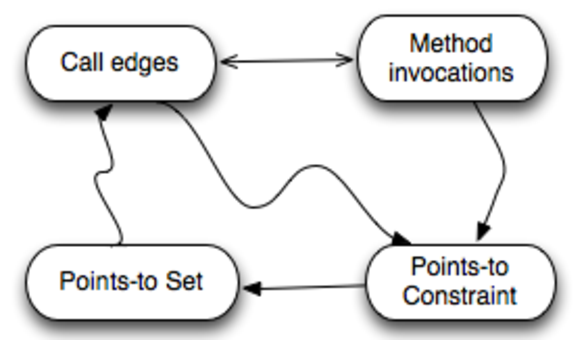
\includegraphics[scale=0.8]{img/callgraph}
\end{center}
\caption{On-the-fly Call graph construction.}
\label{fig-ffsm}
\end{figure}

\begin{figure}
\begin{center}
\inferrule
{Comp(s,m), launch(v,m), pt(v,o), intf(f), pt(f,c), CH(c,t)}
{ICCG(s,t)}
\end{center}
\caption{ICCG construction rule}
\label{fig-ffsm}
\end{figure}

\subsection{Legacy Computation}
We define the legacy of a component $T$ as the properties that is held by $T$. The legacy can be any reachable methods that may lead to potential malicious behaviors, or sources and sinks that are produced in current component $T$, intent filters and permissions, etc.  

Since we already have a precise call graph and ICCG, computing the legacy for each component is pretty straightforward. Please refer to our technical report for more detail.

\subsection{Query Guided Malware Detection}
After previous two steps we will store all the information of ICCG into a database and the next step will be how to construct a query for each specific malware family. In other word, how to quantify the semantic behavior of a malware family.
We formalize the query into a formula which is interpreted by "Kripke Structure"[8]:
\[
<P, S, R, L> 
\]
$P$: Finite set of atomic propositions listed in Table 2 ; \\
$S$: Set of components.\\
$R$: A relation from one component to another; \\
$L$: A label function that maps a component to literals. \\
Type system of query language:
\[
\tau = receiver | activity | service | \top
\]
$\top$ denotes any type of component that is unknown.\\
The example in figure 2, if we denote the receiver as $s$ and service as $t$, a query of checking whether a given application's ICCG matches the behavior of this malware family can be formalized as:
 \[
\begin{array}{cc}
\exists s. \exists t. \tau(s)=receiver \land \text{PHONE\_STATE} \in Filter(s) \\
\land \tau(t)=service \land R(s,t)  \\
\land (\langle \$deviceId, !Internet\rangle \in Flow(t) )
\end{array}
\]
 
$Flow(s)$ maps $s$ to a set of source-sink labels.  It's domain is  all possible source-sink pairs.\\
$Filter(s)$ maps $s$ to a set of intent filters;  It's domain is all possible action strings in Android framework, such as "PHONE\_STATE", "SMS\_RECEIVED".\\
If we want to query whether exists a service which not only has a source-sink from deviceId to internet, but also abort broadcast, the formula will look like this:
\[
\begin{array}{cc}
\exists x. \tau(x)=service \land \\
 (\langle \$deviceId, !Internet\rangle \in Flow(x) )\land p^{x}_{1}
\end{array}
\]
where $p^{x}_i$ denotes component $x$ has predicate $i$;\\
In order to come up with queries which can detect malware precisely, we perform a systematic study on top 9 malware families and describe their behavior in table 1. Then we extract a finite set of suspicious behaviors of the malware based on the reports from anti-virus companies.  Table 2 lists all the properties that can be used to quantify malicious behaviors of those 9 malware families. 

\begin{table*}
\centering

\begin{tabular*}{0.75\textwidth}{@{\extracolsep{\fill} } | l | l | l | l | }
  \hline
  Predicate & Operation & Description \\
  \hline
  $p_1$ & abortBroadcast() & method to block current broadcaster \\
  \hline
 $p_2$ &   Leak sensitive data & Leak deviceId to internet \\
 \hline
  $p_3$ & Install app & Install third-party apk \\
  \hline
  $p_4$ & sendTextmessage() & sending SMS \\
  \hline
 $p_5$ &  receiver or service & Type of component \\
 \hline
  $p_6$ & encryption & Encrypt data \\
  \hline
  $p_7$ & High priority receiver & Register the receiver with high priority\\
  \hline
  $p_8$ & getPackageName() &  Check package installed \\
  \hline
  $p_9$ & setWallpaper() & Change current wallpaper. \\
  \hline
  $p_{10}$ & exec() & Execute a script \\
  \hline
  $p_{11}$ & loadLibrary() & Perform native call \\
  \hline
  $p_{12}$ & DexClassLoader() & Perform native call\\
  \hline
\end{tabular*}
\caption{A non exhaustive list of malicious behaviors.}

\end{table*}

\section{Implementation}
We have implemented the proposed technique on top of STAMP, a framework to analyze android application.

\section{Evaluation}
To evaluate the effectiveness of our technique, we perform experiments on a large set of Android applications.

\subsection{Experimental result on Android Malware Genome Project}
First we run our tool on the 1260 applications Genome Malware Project[6], which contains most of the malware in Google Play and other markets in China and Russia during 2010 and 2011. 

Figure 8 shows the partial result of our latest experiment, for those three families: DroidKungFu3, Anserver and Geinimi, we successfully detect more than 97\% of its corresponding samples. For some families that yield poor result, there are reasons. For ADRD, we only detect 45\% of its samples, one reason is our query for this family is not informative enough to quantify a large portion of applications and another reason is some of the applications  actually do not belong to this family. For BaseBridge, the behavior of this family is special because it requires user to trigger the downloading process to install the actual malware.  A large portion of their original codes do not produce any source and sink and suspicious behavior, that's why we fail.

\begin{figure}
\begin{center}
  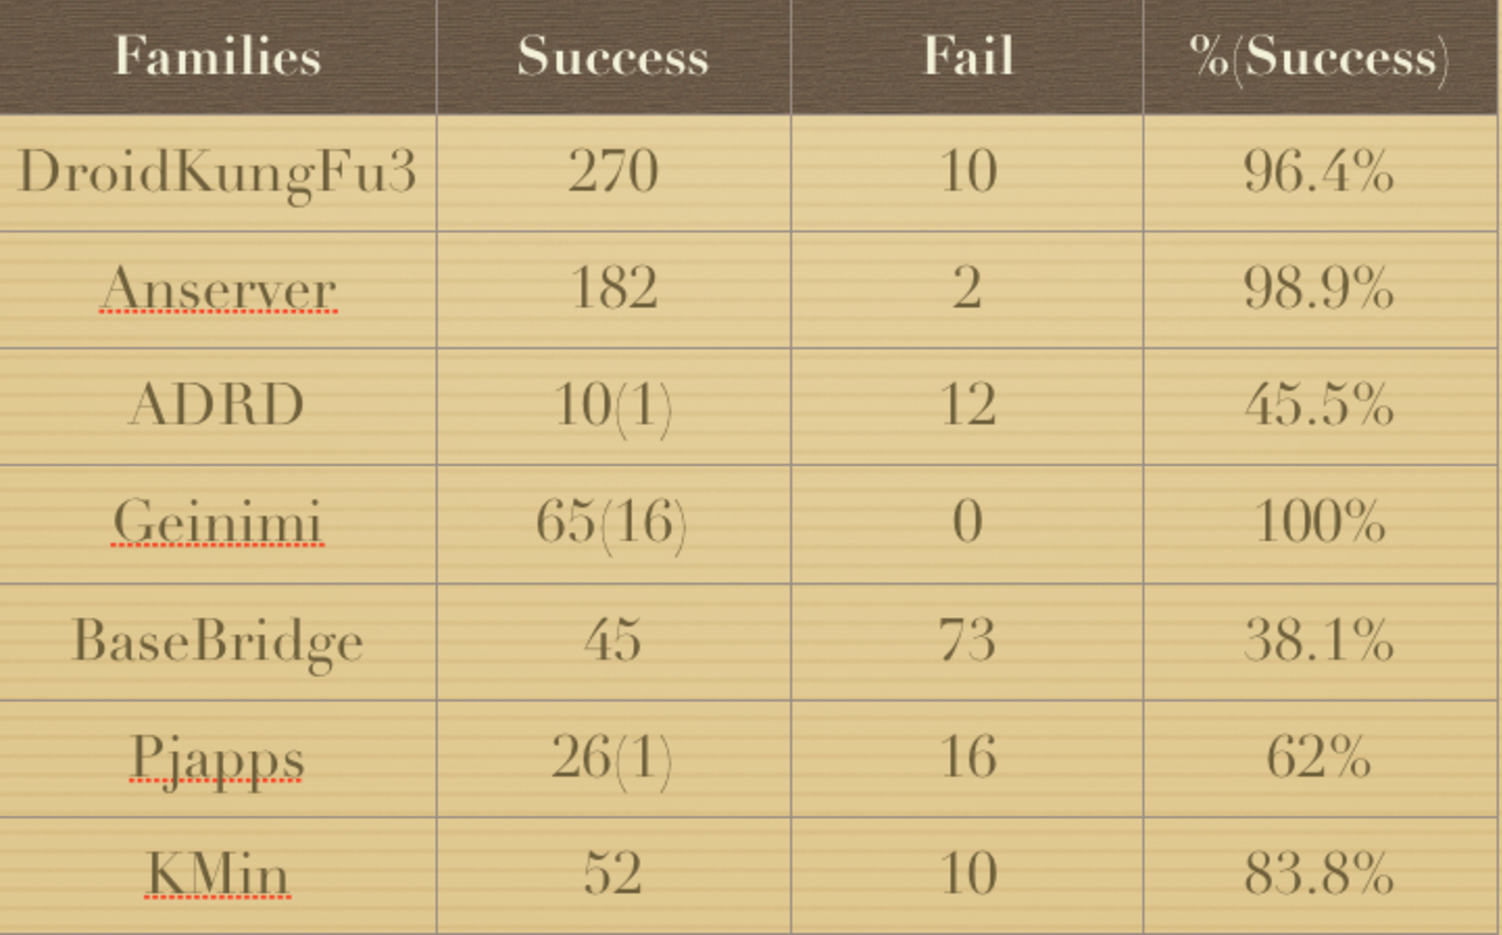
\includegraphics[scale=0.35]{img/genome}
\end{center}
\caption{Result of Genome malware project.}
\label{fig-ffsm}
\end{figure}

\subsection{Experimental result on Google Play}
To verify that our technique does not generate a lot of false positive in those benign applications, we randomly pick up 10, 000 applications in Google Play and run our tool on it.
In Figure 9, for those 418 benign applications that generate output successfully, we only get 2 malware.
\begin{figure}
\begin{center}
  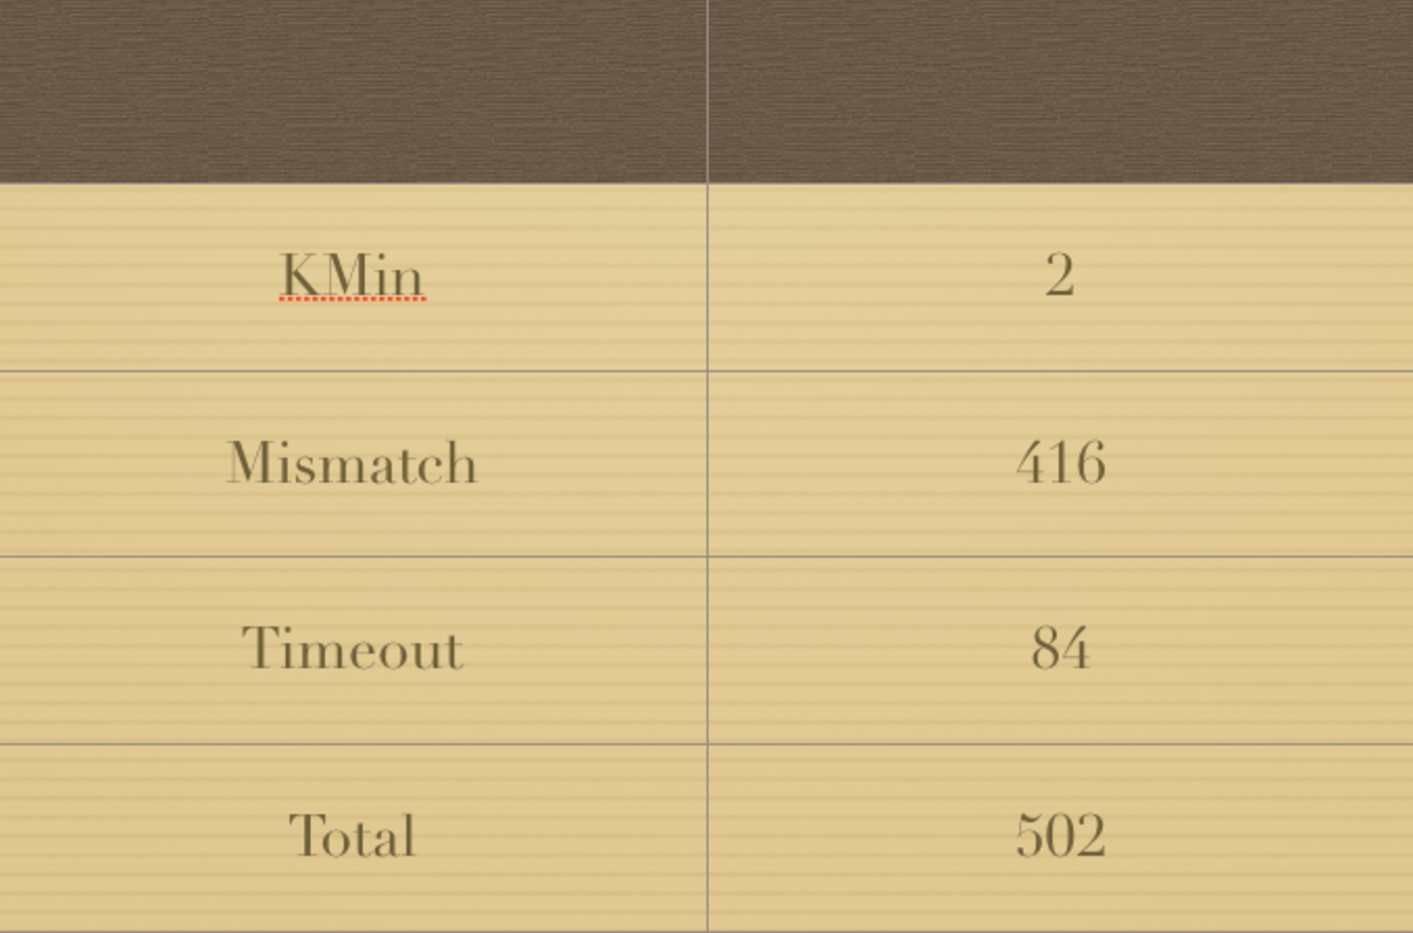
\includegraphics[scale=0.38]{img/googleplay}
\end{center}
\caption{Result of 500 applications in Google Play.}
\label{fig-ffsm}
\end{figure}

\section{Case studies}
TBD.

\section{Related Work}
TBD.

\section{Conclusion and Future Work}
TBD.
%\end{document}  % This is where a 'short' article might terminate

%ACKNOWLEDGMENTS are optional
\section{Acknowledgments}
TBD.

%
% The following two commands are all you need in the
% initial runs of your .tex file to
% produce the bibliography for the citations in your paper.
\bibliographystyle{abbrv}
\bibliography{sigproc}  % sigproc.bib is the name of the Bibliography in this case
% You must have a proper ".bib" file
%  and remember to run:
% latex bibtex latex latex
% to resolve all references
%
% ACM needs 'a single self-contained file'!
%
%APPENDICES are optional
%\balancecolumns
\section{References}

[1] Andersen, Lars Ole. Program analysis and specialization for the C programming language. Diss. University of Cophenhagen, 1994.\\

[2] Sridharan, Manu, et al. "Alias Analysis for Object-Oriented Programs." Aliasing in Object-Oriented Programming. Types, Analysis and Verification. Springer Berlin Heidelberg, 2013. 196-232.\\

[3] Xie, Yichen, and Alex Aiken. "Scalable error detection using boolean satisfiability." ACM SIGPLAN 2005.\\

[4] Kastrinis, George, and Yannis Smaragdakis. "Hybrid context-sensitivity for points-to analysis." PLDI. 2013.\\

[5] Milanova, Ana, Atanas Rountev, and Barbara G. Ryder. "Parameterized object sensitivity for points-to analysis for Java." ACM Transactions on Software Engineering and Methodology (TOSEM) 14.1 (2005): 1-41.

[6] Zhou, Yajin, and Xuxian Jiang. "Dissecting android malware: Characterization and evolution." Security and Privacy (SP), 2012 IEEE Symposium on. IEEE, 2012.

[7] Zhou, Wu, et al. "Fast, scalable detection of Piggybacked mobile applications." Proceedings of the third ACM conference on Data and application security and privacy. ACM, 2013.

[8] Clarke, Edmund M., E. Allen Emerson, and A. Prasad Sistla. "Automatic verification of finite-state concurrent systems using temporal logic specifications." ACM Transactions on Programming Languages and Systems (TOPLAS) 8.2 (1986): 244-263.

[9] https://blog.lookout.com/blog/2011/05/30/security-alert-droiddreamlight-new-malware-from-the-developers-of-droiddream/
% This next section command marks the start of
% Appendix B, and does not continue the present hierarchy
%\balancecolumns % GM June 2007
% That's all folks!
\end{document}
